\documentclass[10pt,a4paper]{article}
\newcommand{\ProductName}{Tandara}
\newcommand{\Slogan}{Tanda Terbaca, Langkah Terjaga}
\newcommand{\TeamName}{Mas Gudegnya Dua Soto Mienya Dua Pakai Nasi}
\newcommand{\TeamLeader}{Husni Abdillah}
\newcommand{\TeamMembers}{Syafran Abdillah Erdin\\Alvian Raihan Ramadan\\Gafna Al Faatiha Prabowo}
\newcommand{\Institutions}{Institut Pertanian Bogor\\Universitas Gadjah Mada}
\newcommand{\ProposalDate}{Oktober 2026}
\newcommand{\AccessDate}{15 Oktober 2026}
\newcommand{\RepositoryRevision}{1c427ab}

\usepackage{styles/tandara}
\begin{document}

% 01 — Cover dari aset pengguna.
\thispagestyle{empty}
\AddToShipoutPictureBG*{\AtPageLowerLeft{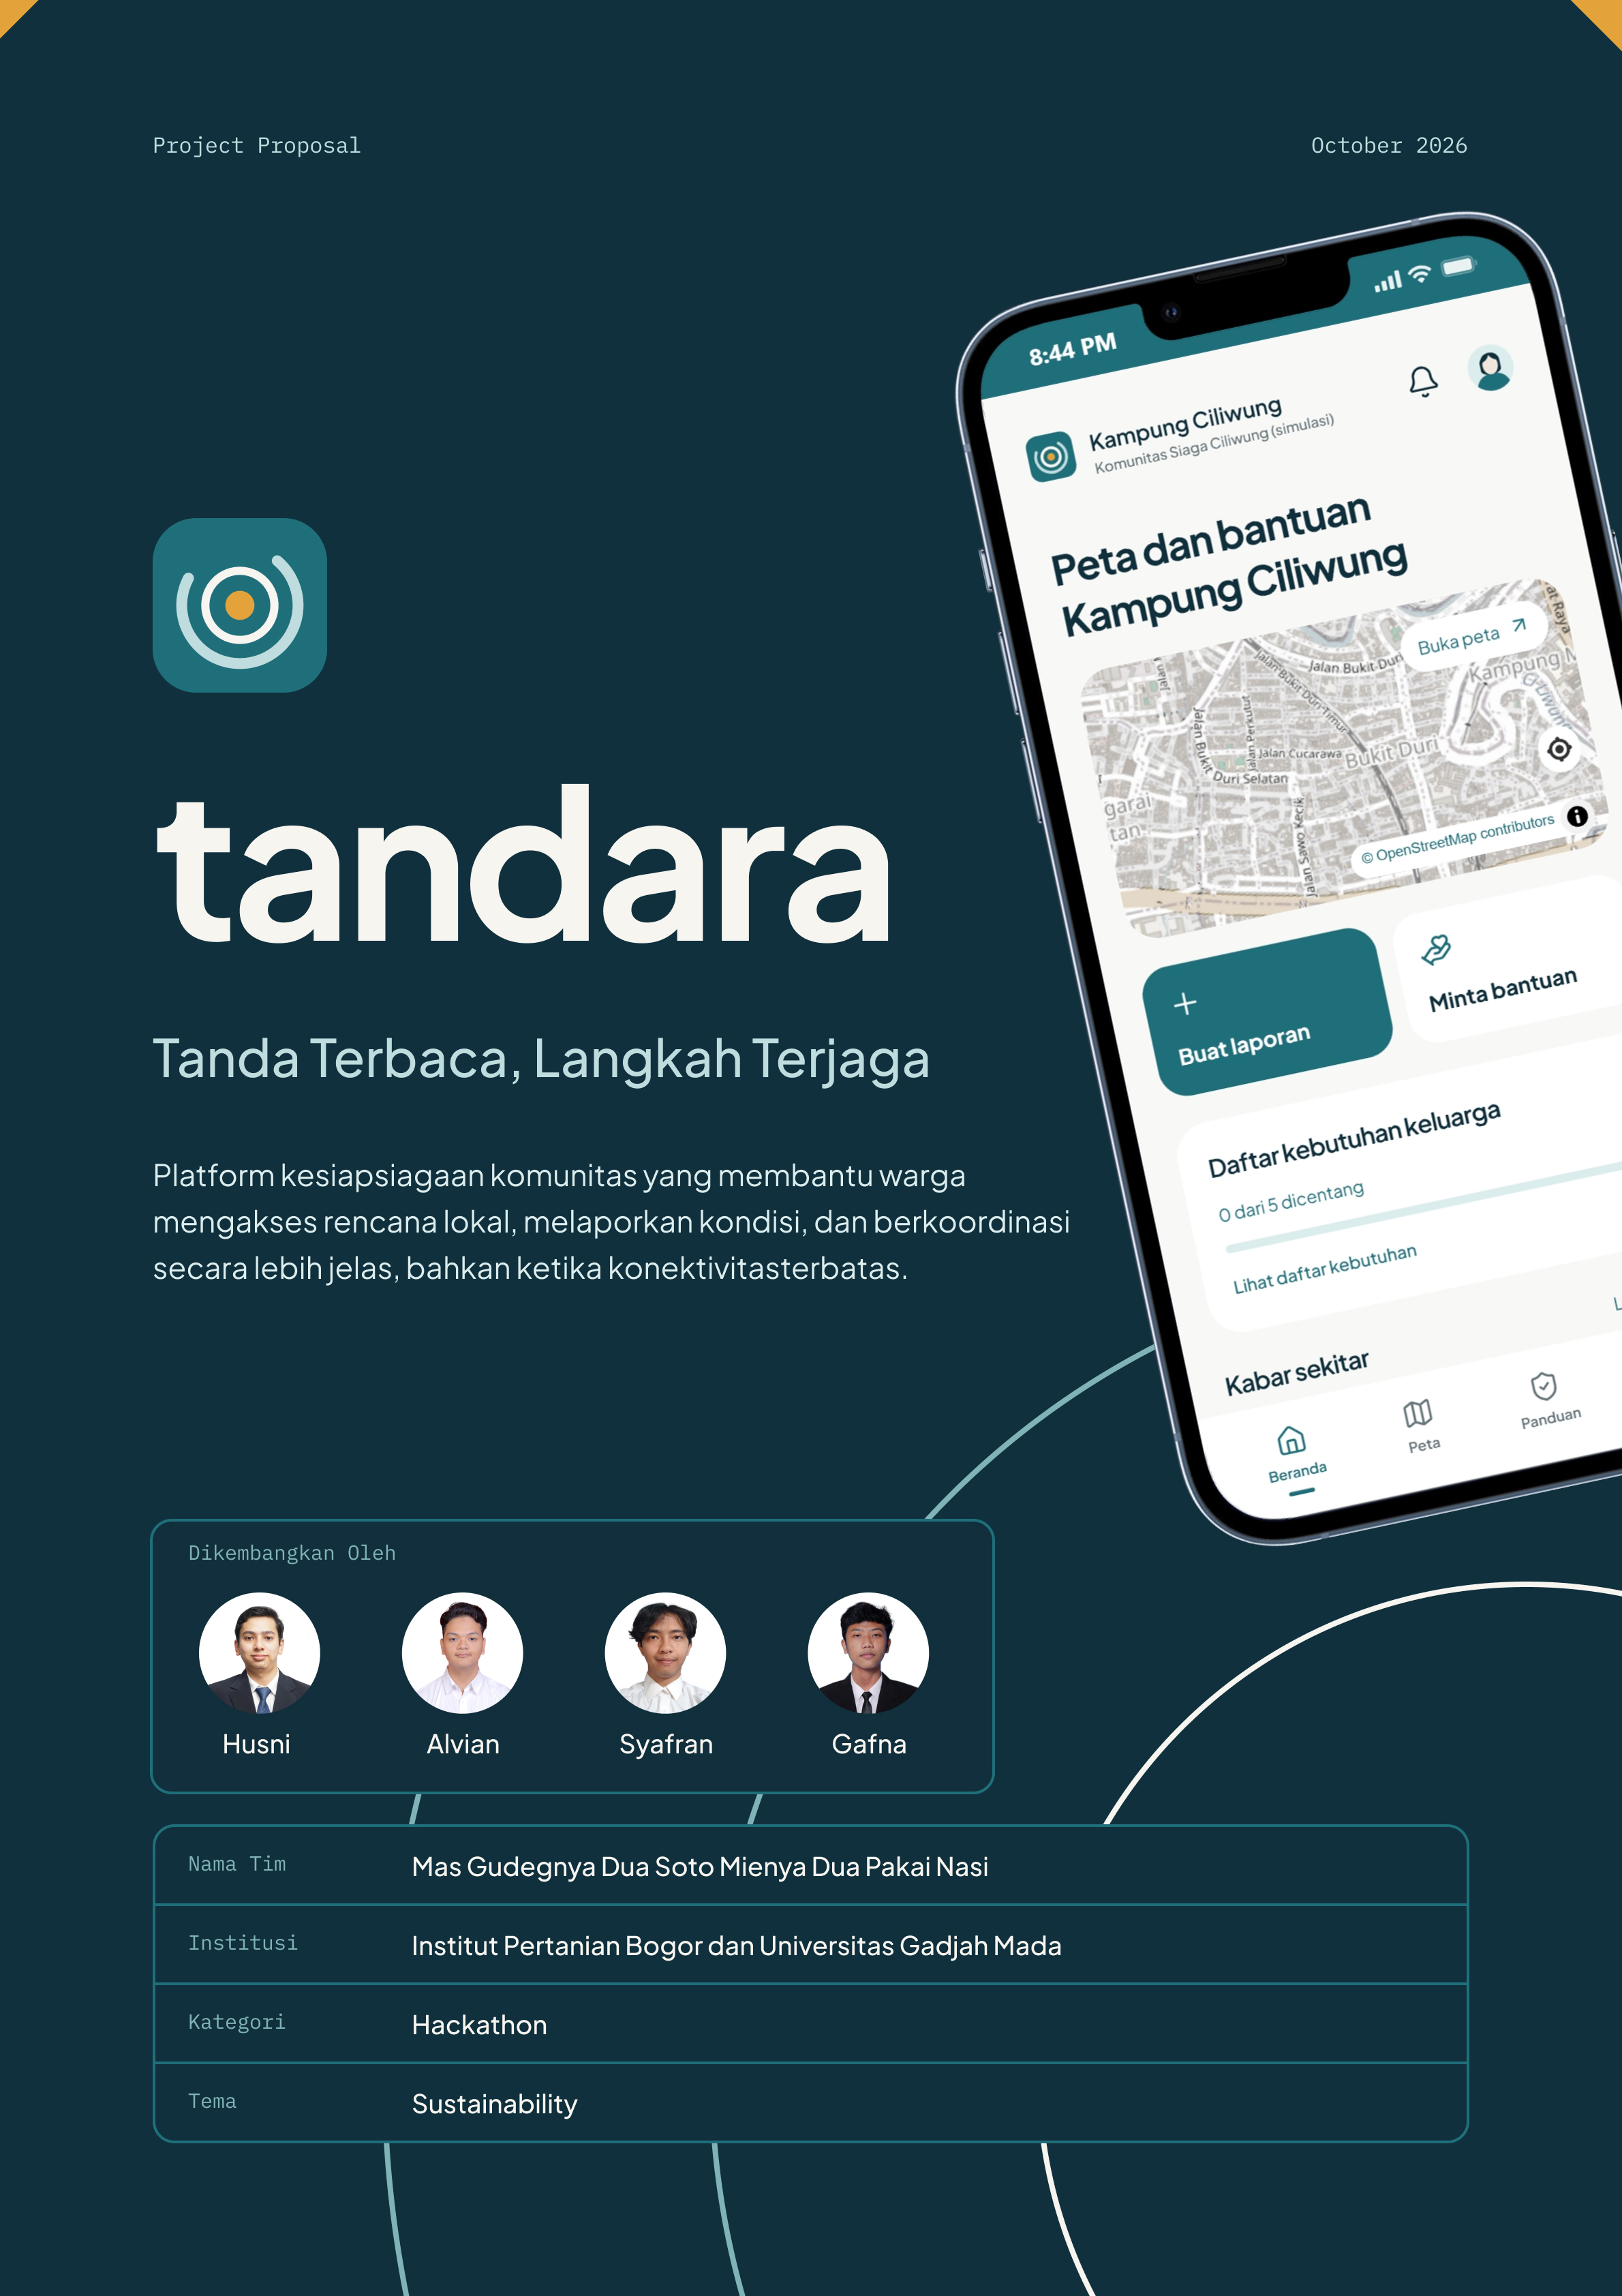
\includegraphics[width=\paperwidth,height=\paperheight]{assets/Proposal · Cover New.jpg}}}
\AddToShipoutPictureFG*{% Correct the final caption line without changing the supplied cover artwork.
% Coordinates follow its 2380 x 3368 px A4 placement; the other lines stay intact.
\begin{tikzpicture}[remember picture,overlay]
  \fill[Deep] ([xshift=54.5bp,yshift=-459bp]current page.north west)
    rectangle ([xshift=250bp,yshift=-471bp]current page.north west);
  \node[anchor=base west,inner sep=0pt,text=Tint,
    font=\fontsize{10.9bp}{14bp}\selectfont]
    at ([xshift=56.25bp,yshift=-469.4bp]current page.north west)
    {bahkan ketika konektivitas terbatas.};
\end{tikzpicture}
}
\null\newpage

% 02 — Ringkasan.
\PageTitle{01 / RINGKASAN EKSEKUTIF}{Kesiapsiagaan yang dekat\newline dengan keseharian warga}{Rencana lokal, informasi bencana, dan laporan warga dalam satu alur.}
Tandara adalah platform kesiapsiagaan komunitas yang membantu warga memahami rencana setempat, menyiapkan kebutuhan keluarga, dan melaporkan kondisi di sekitarnya. Tandara Warga menjadi pintu akses melalui ponsel. Tandara Posko membantu koordinator meninjau laporan dan memperbarui informasi komunitas.

\begin{Callout}
\begin{minipage}[t]{.27\linewidth}\vspace{0pt}\raggedright
{\bfseries\fontsize{31}{36}\selectfont 3.472}\par
\textbf{kejadian bencana}\par Indonesia, tahun 2024
\end{minipage}\hfill
\begin{minipage}[t]{.68\linewidth}\vspace{0pt}\raggedright
BNPB mencatat 1.420 kejadian banjir pada 2024, jenis bencana dengan jumlah kejadian terbanyak pada tahun tersebut. Kesiapan di tingkat rumah tangga dan lingkungan menjadi bagian penting dalam menghadapi risiko bencana~\cite{bnpb2024}.
\end{minipage}
\end{Callout}

\section*{Dari informasi menuju persiapan setempat}
Lindell dan Perry menempatkan penerimaan, perhatian, dan pemahaman informasi sebagai proses awal sebelum penilaian ancaman dan pemilihan tindakan perlindungan~\cite{lindell2012}. Pedoman BNPB menekankan rencana bersama warga, pembagian tanggung jawab, dan latihan untuk kesiapan evakuasi~\cite{bnpbplan}.

\begin{center}\begin{tikzpicture}[x=1mm,y=1mm]
\fill[Tint,rounded corners=3mm] (0,0) rectangle (176,-42);
\foreach \x/\n in {29/01,88/02,147/03}{\fill[Teal] (\x,-6) circle (3.5);\node[font=\ttfamily\fontsize{8}{10}\selectfont,text=white] at (\x,-6) {\n};}
\node[align=center,text width=47mm,font=\fontsize{10}{13}\selectfont] at (29,-23) {\textbf{Informasi tersebar}\\Sumber dan pembaruan\\perlu dikenali};
\node[align=center,text width=47mm,font=\fontsize{10}{13}\selectfont] at (88,-23) {\textbf{Persiapan setempat}\\Rencana, kontak,\\dan kebutuhan keluarga};
\node[align=center,text width=47mm,font=\fontsize{10}{13}\selectfont] at (147,-23) {\textbf{Koordinasi lingkungan}\\Laporan, peninjauan,\\dan tindak lanjut};
\draw[arrow] (54,-23)--(62,-23);\draw[arrow] (113,-23)--(121,-23);
\end{tikzpicture}
\end{center}
\SmallCaption{Gambar 1. Kebutuhan informasi dan koordinasi pada tingkat komunitas.}

\begin{minipage}[t]{.48\linewidth}\vspace{0pt}\raggedright
\subsection*{Cakupan informasi bencana}
Tandara mencakup kebutuhan informasi cuaca, banjir, dan gempa bumi. BMKG menjadi rujukan informasi resmi cuaca dan gempa. Rencana lokal serta laporan warga memberi konteks mengenai kesiapan dan kondisi lingkungan~\cite{bmkgcap,bmkgforecast,bmkggempa}.
\end{minipage}\hfill
\begin{minipage}[t]{.48\linewidth}\vspace{0pt}\raggedright
\subsection*{Pengguna yang dilayani}
Rumah tangga, pengurus RT/RW, relawan, dan koordinator komunitas menjadi pengguna utama. Penyusunan rencana melibatkan lansia, penyandang disabilitas, serta pendamping agar kebutuhan akses dan bantuan tercatat sejak awal.
\end{minipage}

\begin{WhiteBox}
WMO menghubungkan pengetahuan risiko, pemantauan, komunikasi peringatan, serta kesiapsiagaan dan respons dalam satu sistem. Tandara mendukung komunikasi dan persiapan lokal melalui informasi yang mudah ditemukan dan dikelola bersama~\cite{wmo2024}.
\end{WhiteBox}
\newpage

% 03 — Posisi produk.
\PageTitle{02 / KEBUTUHAN DAN POSISI PRODUK}{Informasi resmi terhubung\newline dengan kebutuhan lingkungan}{Tandara melengkapi layanan kebencanaan dan kanal komunikasi yang digunakan warga.}
Informasi bencana tersedia melalui beragam layanan. Pada tingkat lingkungan, warga tetap perlu mengetahui rencana yang berlaku, memahami status laporan, dan menghubungi pengelola setempat. Tandara menyatukan kebutuhan tersebut dalam alur kesiapsiagaan yang dikelola komunitas.

{\fontsize{9.3}{12.5}\selectfont
\begin{tabularx}{\linewidth}{@{}P{25mm}YY@{}}
\toprule\rowcolor{Tint}\textbf{Layanan} & \textbf{Peran utama} & \textbf{Hubungan dengan Tandara}\\\midrule
BMKG & Informasi resmi cuaca, peringatan dini cuaca, dan gempa bumi~\cite{bmkgcap,bmkgforecast,bmkggempa}. & Rujukan informasi resmi dengan sumber serta waktu pembaruan yang ditampilkan jelas.\\
Posko Banjir DSDA & Pemantauan tinggi muka air (TMA) pintu air dan pos pantau~\cite{poskobanjir}. & Data sensor tinggi muka air aktual untuk verifikasi potensi genangan sungai.\\
InaRISK/BNPB & Kajian risiko bencana dan dasar perencanaan wilayah~\cite{inarisk,uu24}. & Rujukan penyusunan rencana kontinjensi dan pengenalan risiko setempat.\\
Laporan warga & Laporan terverifikasi warga setempat dan urun-daya komunitas~\cite{petaapi}. & Konteks langsung kondisi riil lingkungan yang divalidasi koordinator posko.\\
Grup warga & Percakapan dan penyebaran pesan sehari-hari. & Kanal untuk membagikan tautan rencana, pembaruan komunitas, dan ajakan persiapan.\\
Tandara & Rencana lokal, akses offline, laporan terstruktur, dan tinjauan koordinator. & Menghubungkan persiapan warga dengan pengelolaan informasi di tingkat lingkungan.\\\bottomrule
\end{tabularx}}

\SmallCaption{Tabel 1. Peran layanan informasi dan kontribusinya dalam alur kesiapsiagaan.}

\section*{Bekerja bersama grup warga}
Grup WhatsApp mendukung percakapan dan penyebaran pesan sehari-hari. Tandara menambahkan formulir laporan, tanda terima, status tinjauan, serta rencana lokal yang memiliki pemilik dan tanggal peninjauan. Tautan informasi Tandara dapat dibagikan melalui kanal komunikasi yang sudah digunakan warga.

\begin{Callout}
\textbf{Laporan lebih mudah ditelusuri.} Warga dapat melihat perkembangan laporannya melalui tanda terima. Koordinator memperoleh laporan asli, saran ringkasan, dan riwayat penanganan dalam satu tempat.
\end{Callout}

\begin{minipage}[t]{.48\linewidth}\vspace{0pt}\raggedright
\subsection*{Konteks yang mudah dikenali}
Sumber, waktu pembaruan, wilayah, dan status informasi ditampilkan bersama isinya. Informasi resmi dan laporan warga memiliki penanda yang berbeda sehingga lebih mudah dipahami.
\end{minipage}\hfill
\begin{minipage}[t]{.48\linewidth}\vspace{0pt}\raggedright
\subsection*{Persiapan saat koneksi terbatas}
Warga menyimpan rencana sebelum dibutuhkan. Rencana tersimpan dan checklist membantu persiapan ketika akses jaringan terganggu, sebagaimana komunikasi juga dapat terdampak saat bencana~\cite{itu}.
\end{minipage}
\newpage

% 04 — Solusi.
\PageTitle{03 / SOLUSI DAN NILAI PRODUK}{Rencana, laporan, dan tinjauan\newline dalam satu rangkaian}{Alur Tandara menghubungkan persiapan warga dengan pengelolaan informasi komunitas.}
Koordinator menyiapkan rencana lokal bersama pengelola lingkungan. Warga membuka rencana, menyimpan panduan, dan melengkapi checklist persiapan. Saat menemukan kondisi yang perlu diketahui komunitas, warga mengirim laporan untuk ditinjau melalui Tandara Posko.

\begin{center}\begin{tikzpicture}[x=1mm,y=1mm]
\tikzset{flowcard/.style={box,text width=45mm,minimum height=24mm,inner sep=3mm,font=\fontsize{9.5}{13}\selectfont}}
\node[flowcard,fill=Tint,draw=TealSoft] (a) at (27,0) {\textcolor{Teal}{\textbf{01 / BERSIAP}}\\Rencana lokal, checklist,\\dan panduan tersimpan};
\node[flowcard] (b) at (88,0) {\textcolor{Teal}{\textbf{02 / MELAPOR}}\\Pengamatan warga\\beserta konteks lokasi};
\node[flowcard] (c) at (149,0) {\textcolor{Teal}{\textbf{03 / TRIASE}}\\Kategori, ringkasan,\\dan informasi pelengkap};
\node[flowcard,fill=Deep,draw=Deep,text=white] (d) at (149,-39) {\textbf{04 / MENINJAU}\\Koordinator memeriksa\\laporan asli dan saran};
\node[flowcard,fill=Tint,draw=TealSoft] (e) at (88,-39) {\textcolor{Teal}{\textbf{05 / MEMPERBARUI}}\\Ringkasan komunitas\\yang telah ditinjau};
\node[flowcard] (f) at (27,-39) {\textcolor{Teal}{\textbf{06 / MEMELIHARA}}\\Rencana dan persiapan\\diperbarui bersama};
\draw[arrow] (a)--(b);\draw[arrow] (b)--(c);\draw[arrow] (c)--(d);\draw[arrow] (d)--(e);\draw[arrow] (e)--(f);\draw[arrow] (f)--(a);
\end{tikzpicture}

\end{center}
\SmallCaption{Gambar 2. Alur kesiapsiagaan dan pengelolaan laporan Tandara.}

\begin{minipage}[t]{.48\linewidth}\vspace{0pt}\raggedright
\section*{Tandara Warga}
\begin{itemize}
\item Membuka rencana lokal yang memuat panduan persiapan, titik kumpul, kontak, dan catatan akses.
\item Menyimpan rencana untuk dibuka kembali tanpa koneksi dan mencatat checklist di perangkat.
\item Membaca informasi resmi serta pembaruan komunitas dengan sumber dan waktu yang jelas.
\item Mengirim laporan kondisi dan melihat statusnya melalui tanda terima.
\end{itemize}
\end{minipage}\hfill
\begin{minipage}[t]{.48\linewidth}\vspace{0pt}\raggedright
\section*{Tandara Posko}
\begin{itemize}
\item Mengelola rencana berversi beserta pemilik, peninjau, dan masa berlakunya.
\item Membaca laporan asli bersama saran kategori, ringkasan, dan informasi yang perlu dilengkapi.
\item Meminta klarifikasi, mencatat keputusan, dan menyiapkan ringkasan komunitas.
\item Mengelola permintaan bantuan melalui akses terbatas bagi koordinator berwenang.
\end{itemize}
\end{minipage}

\begin{WhiteBox}
\textbf{Pembaruan yang memiliki konteks.} Koordinator meninjau laporan sebelum membagikan ringkasan publik. Tampilan cakupan observasi membantu mengenali area yang memerlukan pembaruan dari warga atau petugas setempat.
\end{WhiteBox}
\newpage

% 05 — Alur pengguna.
\PageTitle{04 / PENGALAMAN PENGGUNA}{Langkah yang jelas\newline bagi warga dan koordinator}{Akses melalui ponsel untuk warga, ruang tinjauan untuk pengelola komunitas.}
\begin{center}\begin{tikzpicture}[x=1mm,y=.8mm]
\tikzset{task/.style={box,text width=32mm,minimum height=14mm,inner sep=2mm,font=\fontsize{8.8}{11.5}\selectfont}}
\fill[Tint,rounded corners=2mm] (0,0) rectangle (176,-24);
\fill[white,rounded corners=2mm] (0,-26) rectangle (176,-50);
\fill[Tint,rounded corners=2mm] (0,-52) rectangle (176,-76);
\node[anchor=west,font=\bfseries\fontsize{9}{12}\selectfont] at (3,-12) {Warga};
\node[anchor=west,font=\bfseries\fontsize{9}{12}\selectfont] at (3,-38) {Sistem};
\node[anchor=west,font=\bfseries\fontsize{8.3}{11}\selectfont] at (3,-64) {Koordinator};
\node[task] (a) at (49,-12) {Buka dan simpan\\rencana lokal};
\node[task] (b) at (97,-12) {Isi checklist\\dan kirim laporan};
\node[task] (c) at (150,-12) {Lihat tanda terima\\dan pembaruan};
\node[task,fill=Tint,draw=TealSoft] (d) at (97,-38) {Simpan laporan\\dan siapkan saran};
\node[task] (e) at (49,-64) {Susun dan terbitkan\\rencana lokal};
\node[task,fill=Deep,draw=Deep,text=white] (f) at (97,-64) {Tinjau laporan\\dan catat keputusan};
\node[task] (g) at (150,-64) {Perbarui status\\atau ringkasan};
\draw[arrow] (e)--(a);\draw[arrow] (a)--(b);\draw[arrow] (b)--(d);\draw[arrow] (d)--(f);\draw[arrow] (f)--(g);\draw[arrow] (g)--(c);
\end{tikzpicture}
\end{center}
\SmallCaption{Gambar 3. Alur warga, sistem, dan koordinator dalam mengelola rencana serta laporan.}

\begin{minipage}[t]{.48\linewidth}\vspace{0pt}\raggedright
\subsection*{Alur Tandara Warga}
Pilih wilayah, buka rencana lokal, simpan panduan, dan lengkapi checklist. Laporan dapat dikirim dengan patokan lokasi berbentuk teks. Tanda terima digunakan untuk melihat perkembangan laporan.
\end{minipage}\hfill
\begin{minipage}[t]{.48\linewidth}\vspace{0pt}\raggedright
\subsection*{Alur Tandara Posko}
Koordinator masuk ke wilayah tugasnya, membuka daftar laporan, lalu memeriksa laporan asli dan saran AI. Hasil tinjauan dicatat sebelum status diperbarui atau ringkasan dibagikan kepada komunitas.
\end{minipage}
\par\vspace{3mm}
\begin{minipage}[t]{.48\linewidth}\vspace{0pt}\raggedright
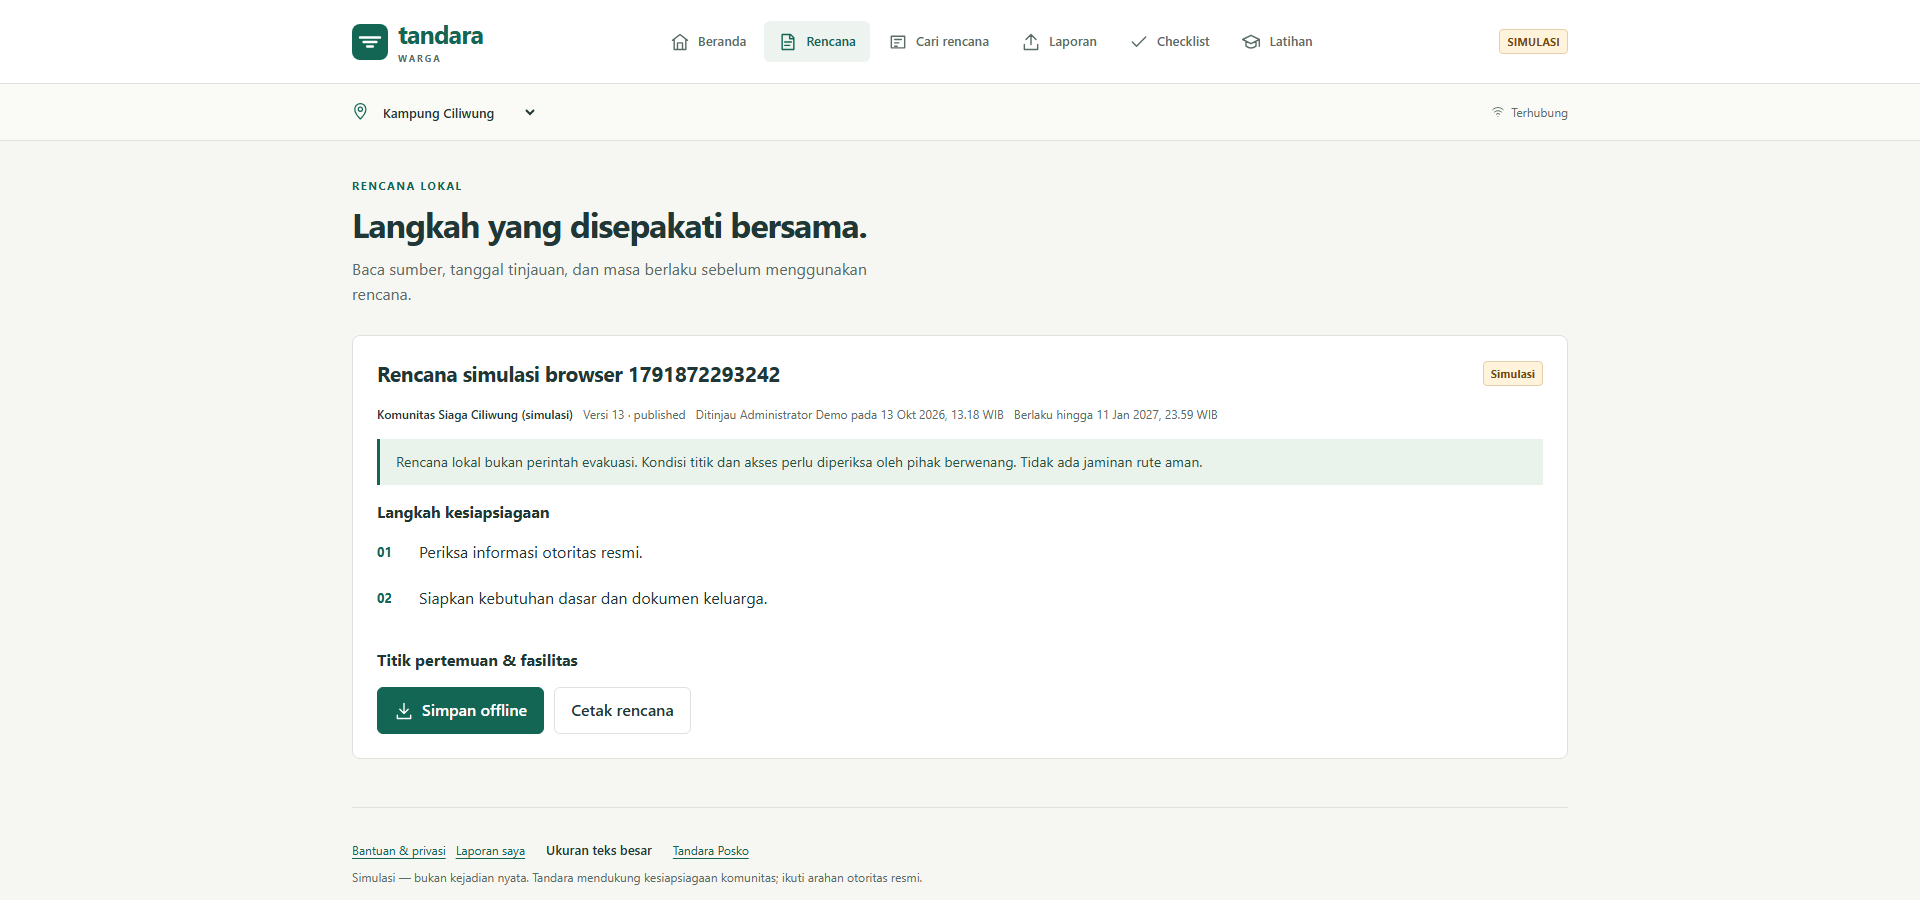
\includegraphics[width=\linewidth,trim=350 135 870 170,clip]{assets/screenshots/warga-plan.png}
\SmallCaption{Gambar 4. Rencana lokal dan pilihan penyimpanan offline pada Tandara Warga.}
\end{minipage}\hfill
\begin{minipage}[t]{.48\linewidth}\vspace{0pt}\raggedright
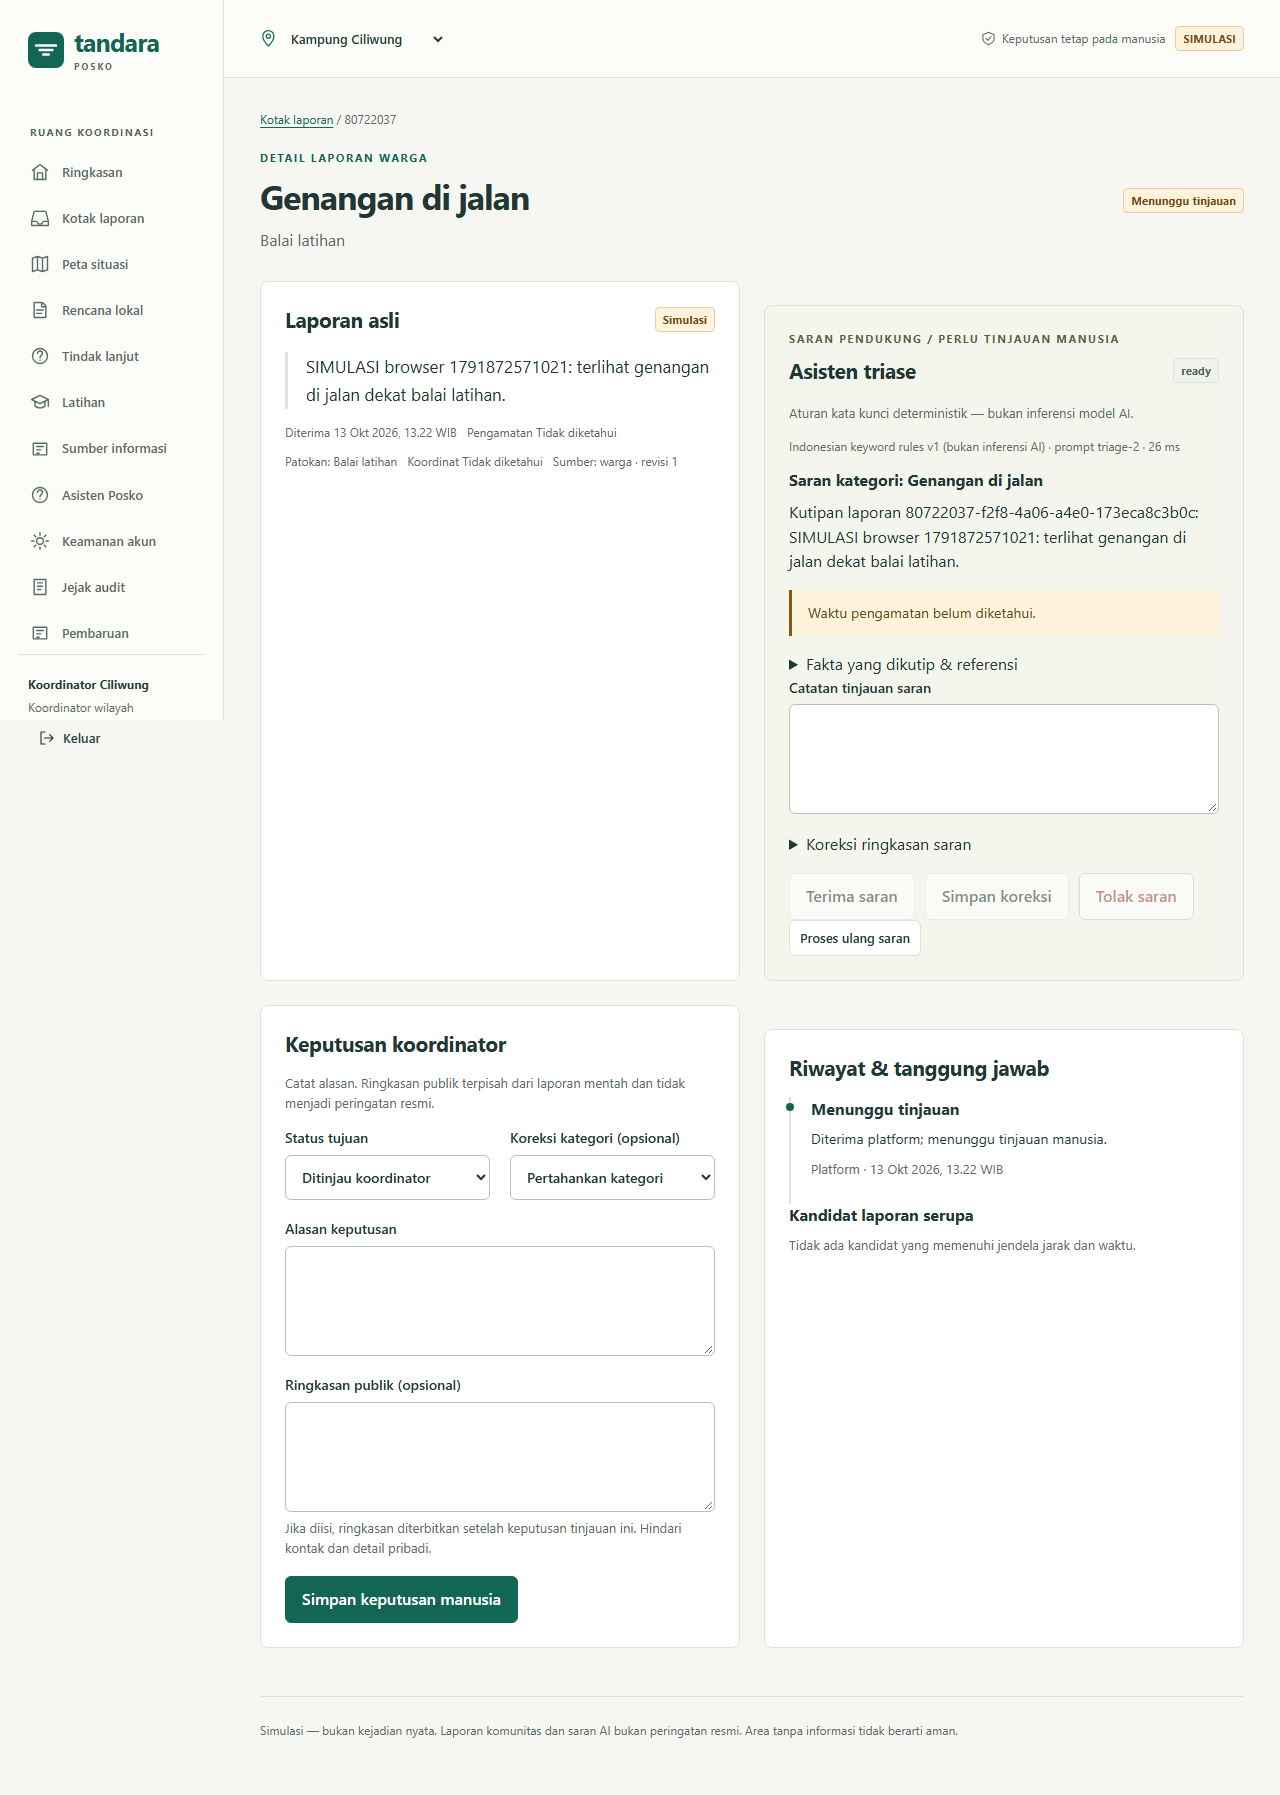
\includegraphics[width=\linewidth,trim=760 1075 30 305,clip]{assets/screenshots/posko-report-detail.png}
\SmallCaption{Gambar 5. Panel saran triase untuk membantu peninjauan laporan pada Tandara Posko.}
\end{minipage}
\newpage

% 06 — AI.
\PageTitle{05 / PENGOLAHAN LAPORAN DAN AI}{Saran triase membantu\newline koordinator membaca laporan}{Kategori, ringkasan, dan informasi yang perlu dilengkapi disajikan bersama laporan asli.}
Laporan warga disimpan terlebih dahulu agar proses penerimaan tetap berjalan. Sistem kemudian menyiapkan saran triase untuk membantu koordinator menyusun prioritas peninjauan. Keputusan dan publikasi ringkasan tetap dilakukan oleh koordinator.

\begin{center}\begin{tikzpicture}[x=1mm,y=1mm]
\tikzset{stage/.style={box,text width=26mm,minimum height=23mm,inner sep=2mm,font=\fontsize{9}{12}\selectfont}}
\node[stage] (a) at (15,0) {\textbf{Terima}\\Validasi\\laporan warga};
\node[stage] (b) at (51,0) {\textbf{Simpan}\\Laporan asli\\dan tanda terima};
\node[stage,fill=Tint,draw=TealSoft] (c) at (87,0) {\textbf{Bantu triase}\\Ringkasan dan\\informasi kurang};
\node[stage,fill=Deep,draw=Deep,text=white] (d) at (123,0) {\textbf{Tinjau}\\Pemeriksaan\\oleh koordinator};
\node[stage] (e) at (159,0) {\textbf{Perbarui}\\Status dan\\ringkasan publik};
\draw[arrow] (a)--(b);\draw[arrow] (b)--(c);\draw[arrow] (c)--(d);\draw[arrow] (d)--(e);
\draw[arrow] (b.south)--++(0,-10)-| (d.south);
\node[note,fill=Paper,inner sep=1.5mm] at (87,-23) {Tinjauan manual tetap tersedia};
\end{tikzpicture}
\end{center}
\SmallCaption{Gambar 6. Pengolahan laporan dengan tinjauan manusia sebelum publikasi.}

\begin{minipage}[t]{.48\linewidth}\vspace{0pt}\raggedright
\begin{WhiteBox}
\Tag{CONTOH PENGOLAHAN LAPORAN}\par
“Air sudah setinggi lutut di jalan dekat balai warga. Motor tidak bisa lewat.”
\par\textbf{Kategori}\par
Akses jalan terdampak.
\par\textbf{Ringkasan}\par
Genangan di dekat balai warga dilaporkan menghambat kendaraan roda dua.
\par\textbf{Informasi yang perlu dilengkapi}\par
Waktu pengamatan dan patokan lokasi yang lebih rinci.
\end{WhiteBox}
\end{minipage}\hfill
\begin{minipage}[t]{.48\linewidth}\vspace{0pt}\raggedright
\subsection*{Tinjauan yang dapat ditelusuri}
Koordinator dapat menerima, mengoreksi, atau menolak saran dengan alasan. Laporan asli dipertahankan agar konteks warga tetap dapat dibaca. Kandidat laporan duplikat diperiksa sebelum ditautkan.

\subsection*{Kualitas saran}
Keluaran terstruktur memisahkan kategori, ringkasan, dan informasi yang kurang. Evaluasi menggunakan laporan berlabel serta pemeriksaan kesesuaian ringkasan dengan teks asli. Pendekatan ini mengikuti kebutuhan pengawasan manusia dalam pengelolaan risiko AI~\cite{nist}.

\subsection*{Pelindungan data}
Permintaan bantuan dan kontak pribadi dibatasi bagi petugas berwenang. Pengelolaan persetujuan, masa simpan, dan penghapusan data mengacu pada UU Pelindungan Data Pribadi~\cite{uu27}.
\end{minipage}

\begin{Callout}
\textbf{AI berperan sebagai asisten triase.} Informasi resmi tetap bersumber dari lembaga berwenang. Instruksi evakuasi dan keputusan lapangan mengikuti otoritas serta pengelola setempat.
\end{Callout}
\newpage

% 07 — Keberlanjutan.
\PageTitle{06 / KEBERLANJUTAN DAN INKLUSIVITAS}{Kesiapan dipelihara\newline bersama komunitas}{Rencana diperbarui, keterampilan dilatih, dan kebutuhan akses dibahas secara berkala.}
Tinjauan sistematis Sufri dkk. menyoroti perlunya keterlibatan komunitas yang berkelanjutan, penggabungan pengetahuan lokal dan ilmiah, serta pelibatan kelompok rentan dalam sistem peringatan dini~\cite{sufri2020}. Pada Tandara, pengelola dan warga memelihara rencana lokal melalui peninjauan serta latihan. Rencana cetak dan pendampingan melengkapi akses aplikasi.

\begin{tabularx}{\linewidth}{@{}P{28mm}YY@{}}
\toprule\rowcolor{Tint}\textbf{Dimensi} & \textbf{Pendekatan} & \textbf{Manfaat yang dituju}\\\midrule
Sosial & Panduan sederhana, checklist, pendampingan, dan akses rencana tersimpan. & Warga lebih mudah memahami persiapan dan menemukan kontak setempat.\\
Kelembagaan & Pemilik rencana, peninjauan berkala, riwayat perubahan, dan serah terima pengurus. & Pengetahuan kesiapsiagaan tetap tersedia ketika pengelola berganti.\\
Adaptasi iklim & Persiapan banjir, latihan lingkungan, serta pembaruan kondisi akses. & Komunitas memiliki kebiasaan persiapan menghadapi bahaya terkait iklim.\\\bottomrule
\end{tabularx}
\SmallCaption{Tabel 2. Kontribusi Tandara terhadap keberlanjutan sosial, kelembagaan, dan adaptasi iklim.}

\begin{center}\begin{tikzpicture}[x=1mm,y=1mm,every node/.append style={inner sep=0pt}]
\draw[TealSoft,line width=1.5pt] (15,0)--(161,0);
\foreach \x/\n in {15/1,51/2,88/3,125/4,161/5}{\fill[Teal] (\x,0) circle (3.5);\node[text=white,font=\bfseries\fontsize{9}{11}\selectfont] at (\x,0) {\n};}
\node[align=center,text width=30mm,font=\fontsize{9}{12}\selectfont,anchor=north] at (15,-7) {Informasi\\mudah dipahami};
\node[align=center,text width=30mm,font=\fontsize{9}{12}\selectfont,anchor=north] at (51,-7) {Persiapan\\rumah tangga};
\node[align=center,text width=30mm,font=\fontsize{9}{12}\selectfont,anchor=north] at (88,-7) {Koordinasi\\lingkungan};
\node[align=center,text width=30mm,font=\fontsize{9}{12}\selectfont,anchor=north] at (125,-7) {Rencana\\terpelihara};
\node[align=center,text width=30mm,font=\fontsize{9}{12}\selectfont,anchor=north] at (161,-7) {Kesiapan\\komunitas};
\end{tikzpicture}
\end{center}
\SmallCaption{Gambar 7. Jalur pengembangan manfaat dari informasi menuju kesiapan komunitas.}

\begin{minipage}[t]{.48\linewidth}\vspace{0pt}\raggedright
\section*{Perencanaan inklusif}
Survei global UNDRR tahun 2023 mencatat bahwa 14\% responden penyandang disabilitas mengetahui rencana pengurangan risiko bencana pada tingkat subnasional. Pelibatan mereka dalam perencanaan menjadi perhatian penting~\cite{undrr2023}.

Tandara mengutamakan bahasa sederhana, status berbentuk teks, dan alternatif daftar untuk peta. Pengembangan aksesibilitas mencakup pengujian pembaca layar, ukuran teks, serta penggunaan bersama pendamping dengan acuan WCAG 2.2~\cite{wcag}.
\end{minipage}\hfill
\begin{minipage}[t]{.48\linewidth}\vspace{0pt}\raggedright
\section*{Keterkaitan dengan SDG}
\textbf{SDG 11}\par
Rencana setempat dan koordinasi warga mendukung upaya pengurangan risiko bencana serta ketangguhan permukiman, terutama target 11.5 dan 11.b~\cite{sdg11}.

\textbf{SDG 13}\par
Persiapan banjir, edukasi, dan latihan komunitas selaras dengan penguatan kapasitas adaptasi serta kesiapsiagaan terhadap bahaya terkait iklim pada target 13.1 dan 13.3~\cite{sdg13}.
\end{minipage}

\newpage

% 08 — Arsitektur.
\PageTitle{07 / ARSITEKTUR DAN KELAYAKAN}{Dua antarmuka,\newline satu alur pengelolaan data}{Arsitektur modular mendukung akses warga, pekerjaan koordinator, dan pengembangan bertahap.}
\begin{center}\begin{tikzpicture}[x=1mm,y=.85mm]
\tikzset{arch/.style={box,text width=67mm,minimum height=22mm,inner sep=2mm,font=\fontsize{9}{12}\selectfont}}
\fill[Tint,rounded corners=3mm] (0,4) rectangle (176,-25);
\node[arch] (w) at (42,-10) {\TechLogo{react}\quad\textbf{Tandara Warga}\\React PWA · Dexie/IndexedDB};
\node[arch] (p) at (134,-10) {\TechLogo{react}\quad\textbf{Tandara Posko}\\React · sesi koordinator};
\node[arch,fill=Deep,draw=Deep,text=white] (api) at (42,-42) {\TechLogo{nestjs}\quad\textbf{API dan otorisasi}\\NestJS · Fastify · Zod · Kysely};
\node[arch] (worker) at (134,-42) {\TechLogo{typescript}\quad\textbf{Worker}\\Triase · sumber · pekerjaan terjadwal};
\node[arch,fill=Tint,draw=TealSoft] (db) at (42,-74) {\TechLogo{postgresql}\quad\textbf{PostgreSQL / PostGIS}\\Laporan · rencana · audit · outbox};
\node[arch] (sources) at (134,-74) {\textbf{Sumber informasi dan AI}\\BMKG · PetaBencana · model AI};
\draw[arrow] (w)--(api);
\draw[arrow] (p.south)--++(0,-2.5mm)-|(api.north);
\draw[arrow] (api)--(db);
\draw[{Stealth[length=2mm]}-{Stealth[length=2mm]},draw=Teal,line width=.8pt] (db.east)--++(10,0)|-(worker.west);
\draw[arrow] (sources)--(worker);
\node[tealbox,text width=170mm,minimum height=10mm,inner sep=2mm,font=\fontsize{9}{12}\selectfont] (infra) at (88,-96) {\TechLogo{docker}\quad\textbf{Infrastruktur}\qquad Docker Compose\quad ·\quad Caddy HTTPS\quad ·\quad VPS};
\end{tikzpicture}
\end{center}
\SmallCaption{Gambar 8. Arsitektur Tandara untuk akses warga, tinjauan laporan, dan pengelolaan informasi.}

{\fontsize{9}{12}\selectfont
\begin{tabularx}{\linewidth}{@{}P{26mm}Y@{}}
\toprule\rowcolor{Tint}\textbf{Lapisan} & \textbf{Teknologi dan peran}\\\midrule
Antarmuka & React, Vite, dan TypeScript untuk aplikasi Warga dan Posko. React Router, TanStack Query, serta Tailwind CSS mendukung navigasi, pengambilan data, dan antarmuka.\\
Akses offline & Dexie/IndexedDB menyimpan rencana, checklist, dan antrean laporan teks. Workbox mendukung pemuatan aplikasi sebagai PWA.\\
Layanan server & NestJS dan Fastify menyediakan API. Zod memvalidasi data, Kysely mengelola query, dan worker menjalankan triase serta pembaruan sumber melalui antrean pekerjaan PostgreSQL.\\
Data dan peta & PostgreSQL menyimpan laporan, rencana, serta riwayat keputusan. PostGIS menangani wilayah dan jarak. MapLibre menampilkan peta dengan atribusi OpenStreetMap~\cite{osmdata}.\\
Operasional & Docker Compose mengemas layanan. Caddy menyediakan akses HTTPS pada VPS. Sesi pengguna dan cakupan wilayah membatasi akses koordinator.\\\bottomrule
\end{tabularx}}

\begin{minipage}[t]{.48\linewidth}\vspace{0pt}\raggedright
\subsection*{Fondasi prototipe}
Prototipe mencakup rencana lokal, checklist, laporan, tanda terima, tinjauan koordinator, dan penyimpanan offline. Struktur bersama menjaga kesesuaian data antara aplikasi Warga, Posko, dan API.
\end{minipage}\hfill
\begin{minipage}[t]{.48\linewidth}\vspace{0pt}\raggedright
\subsection*{Pengembangan sumber informasi}
Integrasi informasi cuaca, gempa, dan tinggi muka air mengikuti format serta atribusi BMKG dan Posko Banjir DSDA DKI. Penyajian sumber menyatukan waktu pembaruan dan konteks wilayah pada pengalaman mobile~\cite{bmkgcap,bmkgforecast,bmkggempa,poskobanjir}.
\end{minipage}
\newpage

% 09 — Roadmap.
\PageTitle{08 / RENCANA PENGEMBANGAN}{Pengembangan bertahap\newline bersama pengelola lokal}{Prioritas dimulai dari alur harian yang utuh dan dilanjutkan dengan perluasan wilayah.}
{\fontsize{9}{12}\selectfont
\begin{tabularx}{\linewidth}{@{}P{28mm}YP{47mm}@{}}
\toprule\rowcolor{Tint}\textbf{Tahap} & \textbf{Fokus kegiatan} & \textbf{Hasil yang dituju}\\\midrule
Hackathon & Menuntaskan integrasi seluruh fungsi inti Warga dan Posko: informasi cuaca, tinggi air dan gempa; rencana lokal, akses offline, pelaporan, dukungan AI, serta tinjauan dan tindak lanjut. & Prototipe terintegrasi siap diuji pada pilot tertutup.\\
Pilot tertutup & Menguji alur bersama 8–12 warga dan 2–3 koordinator; memvalidasi sinkronisasi offline dan navigasi. & Temuan uji dan perbaikan prioritas tervalidasi.\\
Pilot komunitas & Menerapkan alur bersama pengurus RT/RW, menetapkan penanggung jawab, dan simulasi berkala. & Rencana lokal aktif dan prosedur tindak lanjut berjalan.\\
Perluasan wilayah & Menambah komunitas mitra, menguji kapasitas layanan, dan pendampingan pengelola. & Pengelolaan multiwilayah dengan pembagian peran yang jelas.\\\bottomrule
\end{tabularx}
}\SmallCaption{Tabel 3. Roadmap pengembangan Tandara dan hasil pada setiap tahap.}

\section*{Indikator keberhasilan pilot}
{\fontsize{9}{12}\selectfont
\begin{tabularx}{\linewidth}{@{}P{45mm}Y@{}}
\toprule\rowcolor{Tint}\textbf{Indikator} & \textbf{Cara pengukuran}\\\midrule
Kemudahan warga & Target awal minimal 80\% peserta dapat menemukan rencana dan menjelaskan status informasi tanpa bantuan.\\
Keandalan offline & Rencana tersimpan dapat dibuka tanpa koneksi. Antrean laporan tersinkronisasi dengan satu tanda terima per laporan.\\
Pengelolaan komunitas & Seluruh rencana pilot memiliki pemilik, tanggal tinjauan, dan masa berlaku. Waktu peninjauan laporan dicatat.\\
Kualitas saran AI & Penilaian kategori, kesesuaian ringkasan, informasi yang kurang, dan kandidat duplikat menggunakan laporan berlabel.\\\bottomrule
\end{tabularx}}
\SmallCaption{Tabel 4. Ukuran dan target awal untuk evaluasi pilot.}

\begin{minipage}[t]{.48\linewidth}\vspace{0pt}\raggedright
\subsection*{Pengelolaan operasional}
Pengurus menetapkan koordinator, jadwal jaga, dan petugas pengganti. Rencana ditinjau berkala, kontak diperbarui, dan hasil latihan digunakan untuk memperbaiki panduan. Koordinator memeriksa laporan sebelum publikasi serta membatasi akses data bantuan.
\end{minipage}\hfill
\begin{minipage}[t]{.48\linewidth}\vspace{0pt}\raggedright
\subsection*{Keberlanjutan layanan}
Rencana kemitraan diarahkan kepada pengurus lingkungan, pemerintah desa/kelurahan, BPBD, dan organisasi komunitas. Kebutuhan biaya dihitung dari hosting, pencadangan, pemrosesan AI, pelatihan, serta pendampingan pengelola.
\end{minipage}
\newpage

% 10 — Penutup dan pustaka.
\PageTitle{09 / PENUTUP DAN REFERENSI}{Kesiapsiagaan bersama}{Tanda terbaca, langkah terjaga.}
Tandara menghubungkan rencana lokal, persiapan keluarga, dan laporan warga melalui pengelolaan komunitas. Pengembangan bersama pengelola setempat mendukung kesiapsiagaan yang berkelanjutan~\cite{uu24}.

\begin{WhiteBox}[top=2mm,bottom=2mm]
\textbf{Akses produk}\par\vspace{1mm}
{\fontsize{9}{12}\selectfont
\begin{tabularx}{\linewidth}{@{}YY@{}}
\textbf{Tandara Warga} & \textbf{Tandara Posko}\\
\href{https://tandara.my.id/}{\nolinkurl{tandara.my.id}} & \href{https://posko.tandara.my.id/}{\nolinkurl{posko.tandara.my.id}}\\
\addlinespace[1.5mm]
\textbf{Repository} & \textbf{Desain Figma}\\
\href{https://github.com/HusniAbdillah/tandara}{\nolinkurl{github.com/HusniAbdillah/tandara}} & \href{https://ipb.link/product-design-tandara}{\nolinkurl{ipb.link/product-design-tandara}}\\
\end{tabularx}}
\end{WhiteBox}

\vspace{1mm}
{\color{Teal}\bfseries\fontsize{13}{16}\selectfont Daftar pustaka}\par
\begin{multicols}{2}
\printbibliography[heading=none]
\end{multicols}
\end{document}
